\documentclass[main.tex]{subfiles}
\begin{document}
\chapter{Quantum chromodynamics}
\label{chapter:qcd}
\section{Fixed order perturbation theory}
\subsection{NLO QCD}
\section{Divergent structures}
\subsection{Running of the coupling constant}
The behaviour of $\alpha_{\mathrm{s}}$
    is governed by the Callan-Symanzik \cite{Callan:1970yg,Symanzik:1970rt}
    $\beta$-function
    \begin{equation}\label{eqn:beta_fn}
        \mu^{2} \dfrac{\partial \alpha_{\mathrm{s}}(\mu^{2})}{\partial \mu^{2}} = \beta(\alpha_{\mathrm{s}}) \, ,
    \end{equation}
    where the $\beta$-function can be written as a perturbative
    expansion in $\alpha_{\mathrm{s}}$
    \begin{equation}\label{eqn:beta_series}
        -\beta(\alpha_{\mathrm{s}}) = \sum_{n=0}^{\infty}\dfrac{\alpha_{\mathrm{s}}^{n+2}}{(4\pi)^{n+1}} \beta_{n}\, .
    \end{equation}
    where the coefficients $\beta_{n}$ have been computed
    up to fifth order \cite{Baikov:2016tgj,Luthe:2017ttg}.
    The coefficients computed up to this point have been
    strictly positive, meaning that $\alpha_{\mathrm{s}}$
    decreases with increasing energy due to the minus sign
    in (\ref{eqn:beta_series}), a property known as
    asymptotic freedom \cite{Gross:1973id,Politzer:1973fx}.
    The solution to (\ref{eqn:beta_fn}) to first order
    is
    \begin{equation}\label{eqn:1l_alpha}
        \alpha_{\mathrm{s}}(\mu^{2}) = \dfrac{1}{\frac{\beta_{0}}{4\pi}\log\left(\frac{\mu^{2}}{\Lambda_{\mathrm{QCD}}^{2}}\right)} \, ,
    \end{equation}
    where $\Lambda_{\mathrm{QCD}}$ is the QCD scale,
    the scale at which $\alpha_{\mathrm{s}}$ becomes
    large enough that perturbation theory breaks down.
    The running of the coupling constant has been
    observed experimentally as can be seen in Figure~\ref{fig:alpha_s_running}.
    \begin{figure}
        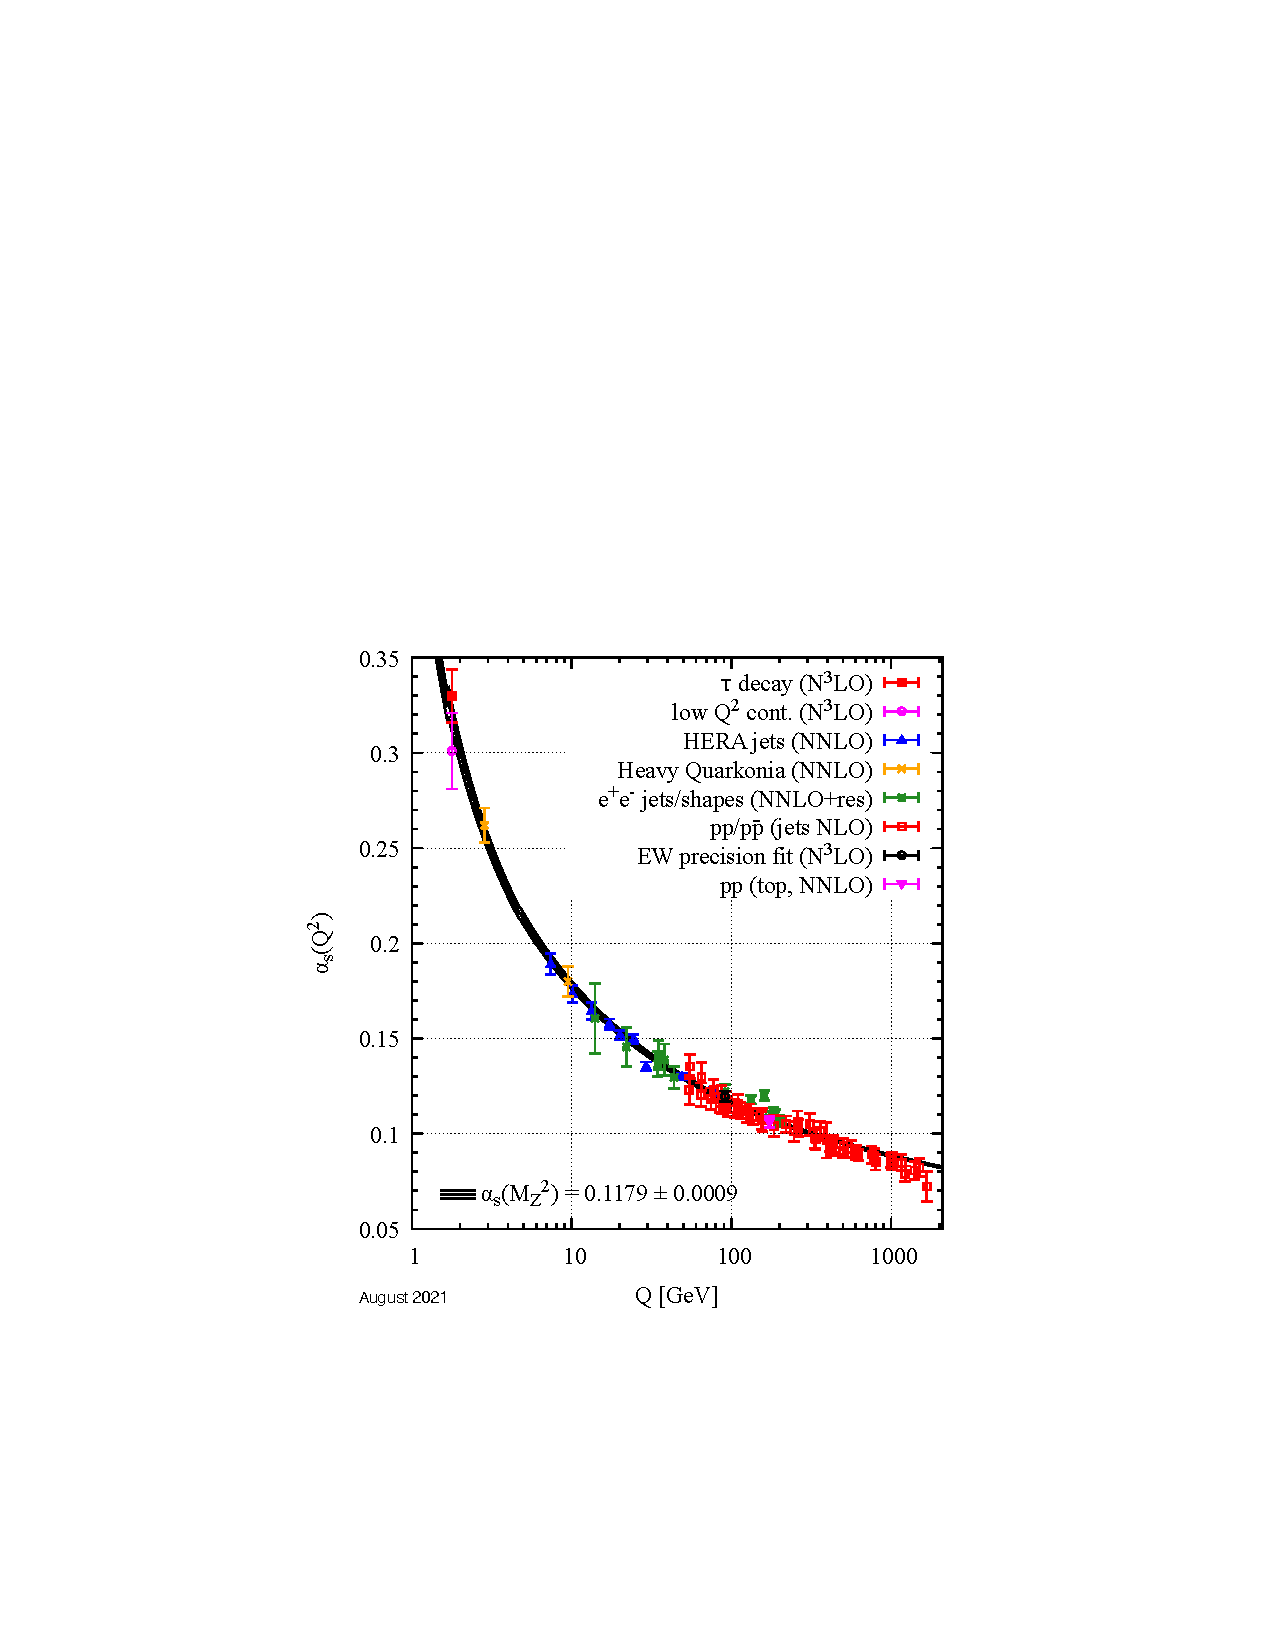
\includegraphics{qcd/alpha_s_running.pdf}
        \caption{The running of the strong coupling constant $\alpha_{\mathrm{s}}$,
        as determined by experiments, with QCD theory prediction in black.
        Figure reference \cite{Workman:2022ynf}.}
        \label{fig:alpha_s_running}
    \end{figure}
    Another consequence of the running coupling
    is colour confinement, in which quarks and
    gluons cannot exist as free particles. Due
    to the increasing strength of coupling at low
    energies, quarks and gluons are forced to
    form composite, colourless particles, known as
    hadrons. The most common example of a hadron
    is the proton which is the origin of the name
    Large Hadron Collider.
\section{Infrared factorisation}
\subsection{Collinear limits}
\subsection{Soft limits}
\section{Subtraction}
\subsection{Catani-Seymour dipoles}
\subsection{Antenna subtraction}
\end{document}